\documentclass[12pt, letterpaper]{article}
\usepackage{amsmath}
\usepackage{amssymb}
\usepackage{graphicx} 
\title{STA 630 - Homework 4}
\author{Anthony Bernardi}
\date{April 9th, 2025}
\begin{document}
\maketitle

\section{Problem 1}

Consider the balanced, additive, one-way ANOVA model: 

\begin{equation}
  Y_{ij} = \mu + \alpha_i + \epsilon_{ij} 
\end{equation} 
\begin{equation}
  i = 1, \dots I, j = 1, \dots, J
\end{equation} 

Where epsilon is normally distributed with parameters ${0, \sigma_{\epsilon}^2}$ iid, with $\mu$, $\alpha_i$ in the real numbers, and $\sigma_{epsilon}^2$ a non-negative number. We adopt the prior structure that is the product of independent conjugate priors, where $\mu$ is a flat prior, alpha is normally distributed, and sigma follows the inverse-gamma distribution with parameters a and b, as we have seen. 

We will assume that $\sigma_{\alpha}^2$ is known, representing the variance of the alpha parameter. We assume a and b for the Inverse Gamma are known as well. 

\subsection{Part a}

Derive the full condition distributions for $\mu$, $\alpha_i$, and $\sigma_{\epsilon}^2$, as required to implement the Gibbs sampler. 

The answer to this question is included on the hand-written sheet. 

\subsection{Part b} 

What is meant by convergence diagnosis? Describe some tools you might use to assist in this regard, what might you do to improve a sampler that is converging slowly?

I would think that, given a Gibbs sampler that is converging slowly, both the starting point of the Gibbs sampling algorithm along with the autocorrelation of the samples would be two factors I would look at first. Given that this is a class of MCMC methods, and these are not independent samples, your starting point matters immensely in evaluating and running your algorithm. Each sample obviously depends on the prior for the full conditionals, so I would evaluate the initial value and starting point when diagnosing a specific Gibbs sampler. 

Looking into the autocorrelation or "stickiness" to use Hoff's term, is what I would evaluate next. If the sampler oscillates between a few values, and doesn't progress throughout the posterior density curve or "mix" well, a sampler with high autocorrelation may be causing this. 

As far as fixing this, picking a different starting point that causes the sampler to mix better may prove beneficial. 

\subsection{Part c} 

Suppose that $\sigma_{\epsilon}^2$ is known. What conditions on the data or the prior might lead to slow convergence for the other parameters via the Gibbs sampler?

I imagine that, if the variance is known, and we are estimating one fewer parameter via Gibbs sampling, we might be "at the mercy" of the now-known variance value, so to speak. If the variance is very small, and the data is very close to the mean, we might have a situation where the posterior density is very peaked around the mean. This would lead to slow convergence, as the sampler would be "stuck" in a small region of the parameter space. 

Largely speaking, a known variance value could be unhelpful in estimating the posterior, in that this might result in different distribution shapes, which could lead to the sampling algorithm being stuck, ultimately obviously slowing convergence. 

\subsection{Part d} 

Some scratch work before completing the Gibbs sampler can also be found in the hand-written notes. 

The R code written in implementing the Gibbs sampler is as follows. 

\begin{verbatim}
# comparing a gibbs sampler for the centered and un-centered algos 
## loading the data 
y <- rnorm(25, 1, 1)
mean.y <- mean(y)
var.y <- var(y)
n <- length(y)

# above serve as likelihoods. Now to the gibbs sampling 
# starting values 
S <- 1000
phi <- matrix(nrow=S, ncol=2)
phi[1,] <- c(mean.y, 1/var.y)
lambda <- matrix(nrow=S, ncol=2) # for the centered case 

# Gibbs sampling algo 
set.seed(1870)
for (s in 2:S){
  # generating the new mean value 
  i <- 1
  mu_n <- rnorm(1, phi[i,1], phi[i,2] / S) # in the matrix 
  i <- i + 1
  phi[i+1,1] <- mu_n 
  
  # other parameter 
  i <- 1
  alpha_n <- rnorm(1, phi[i+1,1], phi[i,2]) # other parameter 
  phi[i+1,2] <- alpha_n
}

# we can now run this and proceed with the algorithm, 
# now we will handle the centered case 
# working with our new parameter matrix 
lambda <- matrix(nrow=S, ncol=2) # for the centered case 

lambda[1,] <- c(mean.y, mean.y + 1/var.y)

for (s in 2:S){
  # generating the new mean as before 
  i <- 1
  mu_n <- rnorm(1, lambda[i,1], lambda[i,2] / S)
  i <- i + 1
  lambda[i+1, 1] <- mu_n
  
  # other parameter 
  i <- 1
  eta_n <- rnorm(1, lambda[i+1, 1], lambda[i,2])
  lambda[i+1,2] <- eta_n 
}
\end{verbatim}

As for which performs better, the parameter case where there is centering compared with where there is not, I would think that the un-centered case performs better, as the centered case is prone to stickiness and limiting its ability to approximate the posterior. 

\section{Problem 2} 

\subsection{Part a} 

After importing the data and some re-arranging, we can do the following to generate a kernel density estimate in R. 

\begin{verbatim}
# reading in the glucose data 
setwd('/home/adbucks/Documents/sta_630/Homeworks/HW4/')
data <- read.table('glucose.dat')
colnames(data) <- "y"

data$y <- as.numeric(data$y)
# now can make our histogram or KDE of the data 
kde <- density(data$y)
plot(kde)
\end{verbatim}

This deviates from the Gaussian in the sense that the symmetry is lacking and the tails are heavier, especially on the right half of the density plot. 

We see the KDE plot in R below. 

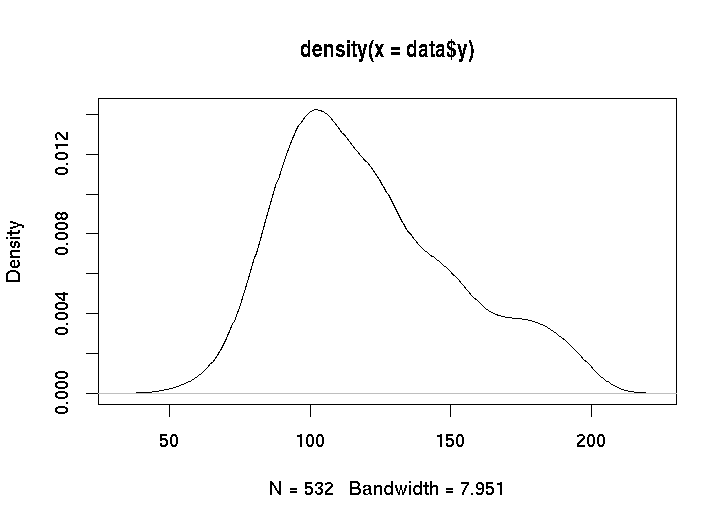
\includegraphics[scale=.75]{../../KDE_plot.png} 

\subsection{Part b} 

In this case, the distributions are listed on the handwritten sheet. 

\subsection{Part c}

With the given initial parameter values, implement a Gibbs sampler with at least 10,000 iterations. 

We can use the min and max values for the theta values to account for the nature of the Gaussian mixed model. 

Compute and plot the autocorrelation functions of the two theta values as well as their effecitve sample sizes. 

Given the initial parameter values, we start to implement the Gibbs sampler with the following R code. 

\begin{verbatim}
# reading in the glucose data 
setwd('/home/adbucks/Documents/sta_630/Homeworks/HW4/')
data <- read.table('glucose.dat')
colnames(data) <- "y"

data$y <- as.numeric(data$y)
# now can make our histogram or KDE of the data 
kde <- density(data$y)
plot(kde)

# now we can try and implement the gibbs sampler with some 
# pre-defined constraints 
a_0 <- 1
b_0 <- 1
mu_0 <- 120
tau_0 <- 200
s_0 <- 1000
rho_0 <- 10
G <- 10000 # number of iterations 

# we can start with the data 
mean_x <- mean(data$y)
var_x <- var(data$y)
n_0 <- length(data$y)

# we start with an initial beta value and then envoke our 
# mixture model 
set.seed(42)

# setting up a parameter matrix 
phi_4 <- matrix(nrow=G, ncol=3)
phi_4[1,] <- c(mean_x, 1/var_x, rho_0)


for (g in 1:G){
  # generating initial values 
  i <- 1 
  beta_s <- rbeta(1, a_0, b_0)
  i <- i + 1
  p <- beta_s
  
  # updating mu 
  mu_n <- rnorm(1, mu_0, s_0)
  mu2_n <- rnorm(1, mu_0, s_0)
  
  # not sure how to incorporate the beta 
  # and the actual mixture 
  
}
\end{verbatim}

I'm unsure as to how to implement the Gibbs sampler with regards to a mixture model. I think that a beta value will have to be sampled first, and then the theta values and finally the variance parameters and components. 

Alternatively, we can initialize the Gibbs sampler by picking a naive p value of .5, and then using the Gibbs sampler to update the parameters of the beta distribution and the p value itself as it integrates with the Gaussian mixture model. 

I know theoretically how this would work, but I'm not totally sure how to implement this with the Gaussian mixture model. 






























\end{document}
